\section{Research questions}

%\section{Future work}

%%%%%%% Measurement approache
\begin{frame}[noframenumbering]
  \frametitle{Approach}
  \begin{itemize}
   \item Naxsi isolation
     \begin{itemize}
       \item Baseline performance measurement (HTTP 200 OK)
       \item URL parameter increments
     \end{itemize}
   \item Real-life scenario
     \begin{itemize}
       \item Baseline performance measurement
       \item Normal usage case
     \end{itemize}
  \end{itemize}
\end{frame}

%%%%%%% HTTP 200 OK: baseline performance measurement
\begin{frame}[noframenumbering]
  \frametitle{HTTP 200 OK: baseline performance measurement}
  \begin{figure}[H]
  \centering
  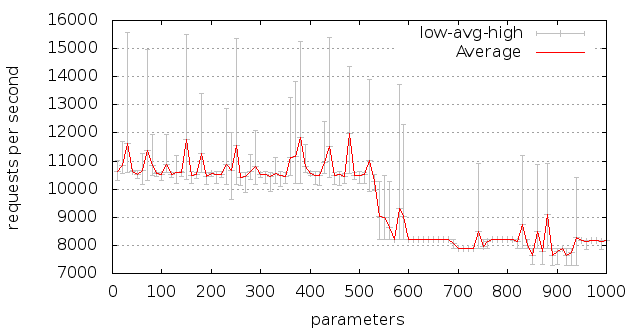
\includegraphics[scale=0.5] {../paper/images/results/baseline_200/output.png}
  \end{figure}
\end{frame}

%%%%%%% HTTP 200 OK: URL allowed paramter increments
\begin{frame}[noframenumbering]
  \frametitle{HTTP 200 OK: URL allowed parameter increments}
  \begin{figure}[H]
  \centering
  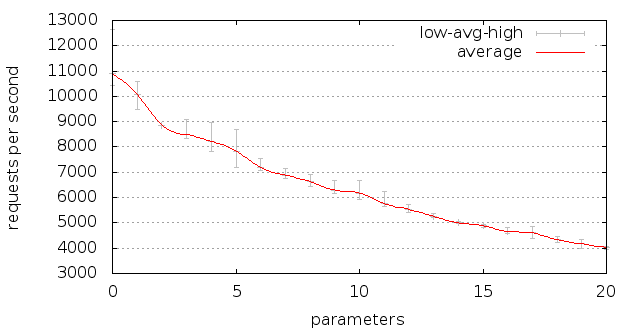
\includegraphics[scale=0.5] {../paper/images/results/200_with_naxsi_incremented_allowed_parameters/output.png}
  \end{figure}
\end{frame}

%%%%%%% HTTP 200 OK: URL disallowed paramter increments
\begin{frame}[noframenumbering]
  \frametitle{HTTP 200 OK: URL disallowed parameter increments}
  \begin{figure}[H]
  \centering
  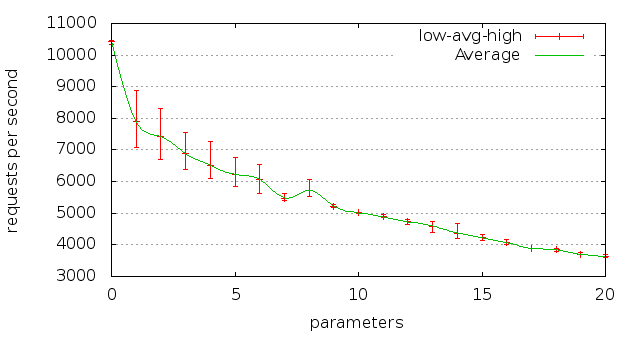
\includegraphics[scale=0.5] {../paper/images/results/200_with_naxsi_incremented_disallowed_parameters/output.png}
  \end{figure}
\end{frame}

%%%%%%% Wordpress baseline
\begin{frame}[noframenumbering]
  \frametitle{Wordpress baseline performance measurement}
  \begin{figure}[H]
  \centering
  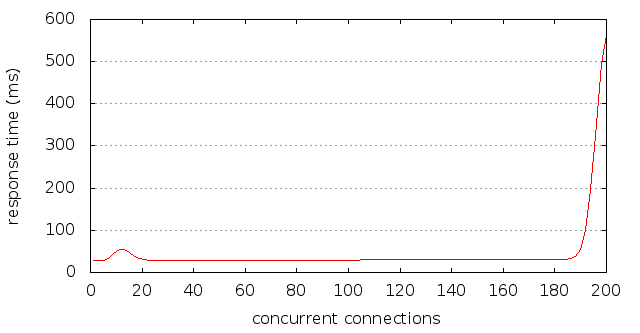
\includegraphics[scale=0.5] {../paper/images/results/baseline_wp/output.png}
  \end{figure}
\end{frame}

%%%%%%% Wordpress with Naxsi
\begin{frame}[noframenumbering]
  \frametitle{Wordpress with Naxsi}
  \begin{figure}[H]
  \centering
  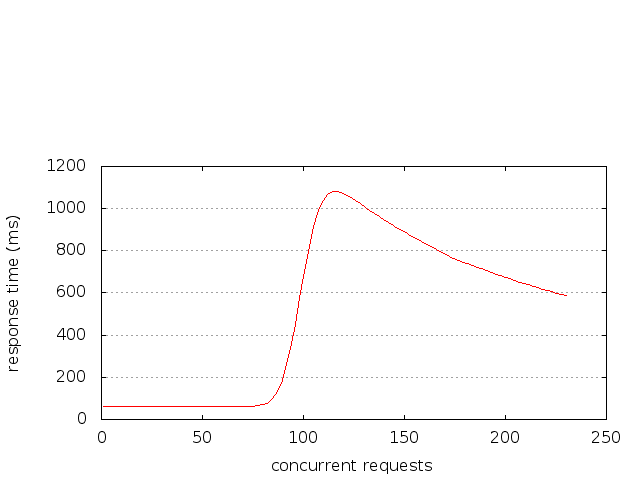
\includegraphics[scale=0.5] {../paper/images/results/wp_with_naxsi_1_to_230_concurrent_connections/output.png}
  \end{figure}
\end{frame}  
  
%%%%%%% Conclusion
\begin{frame}[noframenumbering]
  \frametitle{Conclusion}
  \begin{itemize}
    \item Naxsi has a low overhead
  \end{itemize}
\end{frame}